Разрабатываемый в данном курсовом проекте узел состоит из нескольких логических частей: устройства управления (УУ), трехразрядного регистра режима и непосредственно формирователя импульсной последовательности. Структурная схема приведена на рис. \ref{fig:structure}.\\

\begin{figure}
  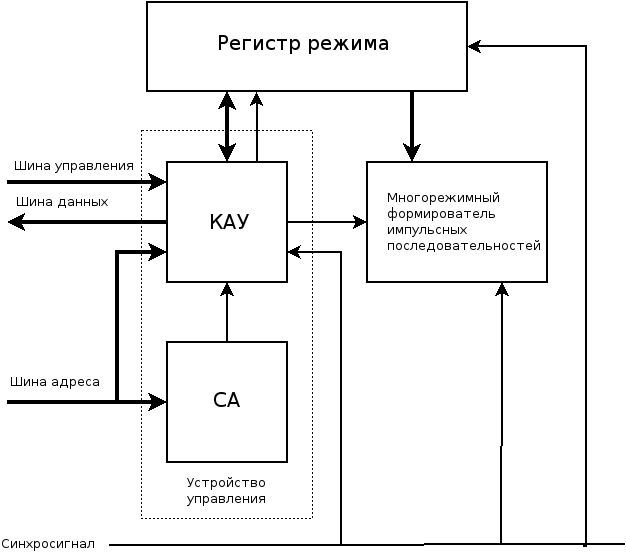
\includegraphics[scale=0.58]{./structure.png}
  \caption{Структура узла. СА - селектор адреса, КАУ - конечный автомат управления.}
  \label{fig:structure}
\end{figure}

Для корректной работы устройства должны присутствовать:
\begin{itemize}
\item Шина данных (ШД)
\item Шина управления (ШУ)
\item Шина адреса (ША)
\item Тактирующий сигнал
\end{itemize}

Подробное описание интерфейса разрабатываемого устройства и протокол его работы представлены в разделе <<Разработка интерфейса сопряжения схемы узла с процессорной системой>>

Устройство управления представляет собой интерфейс узла, через который осуществляется всё взаимодействие с внешним миром. УУ включает в себя селектора адреса и конечный автомат управления. Селектор адреса (СА) читает шину адреса (ША) и при поступлении адреса из нужного диапазона (0x30-0x35) формирует сигнал разрешения. При разрешении от СА, конечный автомат управления (КАУ) может работать. КАУ читает шину управления (ШУ) и реагирует на следующие сигналы от неё: \\